\chapter{Middle Chinese}\label{chapter-3.-Middle-chinese}

The internal reconstruction of Middle Chinese provides a bedrock upon
which all efforts to elucidate Old Chinese phonology build. The Middle
Chinese phonological system exhibits several imbalances and asymmetries.
Each such infelicity affords an opportunity for internal
reconstruction. The nature of internal reconstruction as a method
dictates that a complex attested system descend from an elegant
precursor. One may thus \emph{a priori} guess that the phonology of Old
Chinese achieved through internal reconstruction is simpler than the
true state of affairs. With this danger of oversimplification in mind,
after the internal reconstruction reduces the number of distinct Old
Chinese phonological units relative to Middle Chinese, it is necessary
to consider evidence that Old Chinese maintained distinctions lost in
Middle Chinese.

The term `Middle Chinese' refers to the phonological representation of
Chinese characters as reflected in the 隋 Suí dynasty rime book, the
切韻  \emph{Qièyùn}, written in 601 CE by 陸法言 Lù Fǎyán.\footnote{The
  601 edition is extant only in fragments from Dūnhuáng and Turfan. The
  earliest available complete derivative work is 王仁昫 Wáng Rénxù's
  刊謬補缺切韻  \emph{Kānmiù Bǔquē Qièyùn} of 706 CE (see 
  \cite[62]{Chang1974}, \cite{Takata2004}, and 
  \cite{Bottero2013}). The exposition here generally makes
  reference to the  \emph{Qièyùn}, glossing over differences between it
  and later derivative works. Chinese historical phonology has typically
  relied on the substantially later 廣韻  \emph{Guǎngyùn} of 1007-1008
  (\cite[16-20]{Baxter2014OldChinese}).} Scholars ubiquitously approach the
description of the categories reflected in the  \emph{Qièyùn} through the
rime tables of the 宋 Sòng dynasty, most famously the 韻鏡
 \emph{Yùnjìng} published by 張麟之 Zhāng Línzhī in 1161, but the 七音略
 \emph{Qīyīnlüè}, which appeared the same year in the 通志 \emph{Tōngzhì}
encyclopedia by 鄭樵 Zhèng Qiáo, is also influential. The
in­ter­pre­ta­tion of these sources is complex and con­tro­versial (cf. \cite{Branner2000c},
\cite[8-20]{Baxter2014OldChinese},
\cite{Handel2014},
\cite{jacques17traditional}).

Employing Chinese data for the purposes of comparative linguistics does
not require mastery of these texts and their philology; the Middle
Chinese transcription system of William Baxter 
\citeyearpar[27-86]{Baxter1992}
mechanically reflects all distinctions made in the analysis of the
 \emph{Qièyùn}. Although some effort is made here to explain the meaning
of Baxter's conventions, these details are not relevant for comparative
Trans-Himalayan research. In practice, transcriptions into Baxter's
system are useable as a romanization of philologically attested primary
data, the same function served by the translit­er­a­tion into Roman
letters of the Tibetan or Burmese alphabets. The reader willing to
accept Baxter's transcription at face value may skip ahead to 
\ref{par:rhymes-of-the-Shijing}.

\paragraph{Structure of the \emph{Qièyùn}}.
The four tone categories of Middle Chinese serve as the overarching
principle for the  \emph{Qièyùn}'s organization. The dictionary is
divided into five volumes, with two volumes for characters in the Middle
Chinese level tone (平聲  \emph{píngshēng}) and one each for the rising
(上聲  \emph{shǎngshēng}), departing (去聲  \emph{qùshēng}) and entering
(入聲  \emph{rùshēng}) tones. The terms for these four tone categories,
coined by 瀋約 Shěn Yuē (441-513 CE) and 週顒 Zhōu Yóng (fl. 6c. CE)
(cf. \cite[304]{Baxter1992}), are in Middle Chinese each an example of the
tone in question: 平  \emph{píng} (MChi.  \emph{bjaeng} `level'), 上
 \emph{shàng} (MChi.  \emph{dzyangX} `rising'), 去  \emph{qù} (MChi.
 \emph{khjoH} `de­part­ing'), and 入  \emph{rù} (MChi.  \emph{nyip}
'entering'). In Baxter's system the capital letters -\emph{X} and
-\emph{H} represent the `rising' and `departing' tones respectively.
Both the `level' and `entering' tones are re­pre­sented with no final
capital letter, but a syllable in the `entering' tone ends with a final
stop whereas a syllable in the `level' tone is either open or ends with
a nasal.

The  \emph{Qièyùn} divides the characters classed under each tone into a
total of 193 rime categories (韻目~ \emph{yùnmù}) (cf. §). Within each
rime category those characters with homophonous readings appear
together. These homophone groups (小韻  \emph{xiǎoyùn} or 紐  \emph{niǔ})
are the smallest unit of the work's organization. The pronunciation
of the characters in a single homophone group are presented using
the反切 `\emph{fǎnqiè}' method traditionally credited to 孫炎 Sūn Yán
(220--280 CE) but perhaps used by the earlier scholars Yìng Shào 應劭
(140-206 CE) and 服虔 Fú Qián (late 2nd century) 
\citep[38]{Branner2000c}. The
 \emph{fǎnqiè} method represents a character's pronunciation by
giving two further characters; the first character shares the same onset
as the character annotated and the second character has the same rime as
the character annotated.\footnote{I use `onset' in this setting to
  indicate the phonetic quality shared by the reading of a character and
  the reading of the first of its two  \emph{fǎnqiè }spellers (反切上字
   \emph{fǎnqiè shǎngzì} hereafter `\emph{fǎnqiè} onset spellers'). As
  described below, assuming that the sameness of this relationship is
  transitive `onset' becomes equivalent to 聲類  \emph{shēnglèi}. I
  reserve `initial' for sets of `onsets' in complementary distribution.
  Although not equivalent `onset' is thus closer to an allophone whereas
  `initial' is closer to a phoneme.} To give a concrete example, the
character 東  \emph{tuwng} is glossed with 德 \emph{tok} and 紅
 \emph{huwng}, where the pro­nun­ci­a­tion \emph{tuwng} has the initial
of \emph{t}- of 德  \emph{tok} and the rime -\emph{uwng} of 紅
 \emph{huwng}; one can represent this relationship an equation: 東
 \emph{tuwng} = 德 \emph{t}(\emph{ok}) + 紅 (\emph{h})\emph{uwng}. The
analysis of the pro­nun­ci­a­tion of `fake' as \emph{f}(\emph{old}) +
(\emph{c})\emph{ake}, is an analogous use of the  \emph{fǎnqiè} method in
English.

shows the opening of the opening of the first \emph{píngshēng} volume of
the  \emph{Qièyùn} as it appears in a Dūnhuáng fragment, which lists the
first 18 of the 54 rimes of this volume together with the  \emph{fǎnqiè}
spellings of the names of the rime categories. Note that the first rime
category is 東  \emph{tuwng}, which is given the  \emph{fǎnqiè} spellings
 \emph{tuwng} = 德  \emph{t}(\emph{ok}) + 紅 (\emph{h})\emph{uwng}. shows
two homophone groups from the 刊謬補缺切韻  \emph{Kānmiù Bǔquē Qièyùn} of
706 CE (\cite[7]{Long1968}, 
\cite[49]{Zhou1983}).

\begin{figure}
    \centering
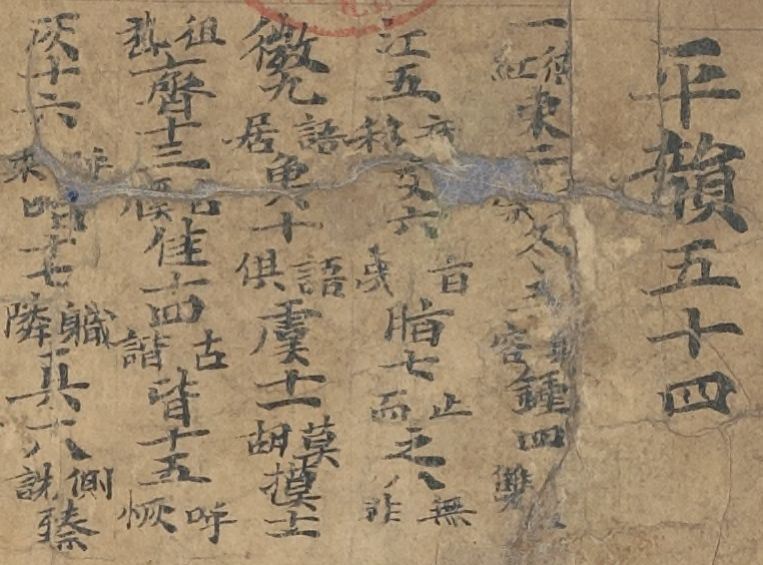
\includegraphics[width=0.90\textwidth]{Chapter5/fig12a P Chin 2017.jpg}
    \caption{Opening of the \emph{Qièyùn} from a Dūnhuáng fragment (PChin. 2017).}
    \label{fig:PChin}
\end{figure}


\begin{figure}[ht]
    \centering
%\begin{minipage}{0.4\columnwidth}
        \begin{tabular}{llll}
Transcription &  \multicolumn{3}{c}{Translation}
 \\
 {\large 平韻五十四}
 &
\multicolumn{3}{c}{There are 54 level tone rimes}
 \\
{\large 一}德紅{\large 東}

& 1. 東 tuwng 
& =
德 \textit{t(ok)}
& +
紅 \textit{(h)uwng} \\
{\large 二}都宗{\large 冬}

& 2. 冬 \textit{towng}
& =
都 \textit{t(u)}
& +
宗 \textit{(ts)owng} \\
{\large 三}職容{\large 鐘}

& 3. 鐘 \textit{tsyowng}
& =
職 \textit{tsy(ik)}
& +
容 \textit{(y)owng} \\
{\large 四}古雙{\large 江}

& 4. 江 \textit{kaewng}
& =
古 \textit{k(uX)}
& +
雙 \textit{(sr)aewng} \\
{\large 五}章移{\large 支}

& 5. 支 \textit{tsye}
& =
章 \textit{tsy(ang)}  
& +
移 \textit{(y)e} \\
{\large 六}旨夷{\large 脂}

& 6. 脂 \textit{tsyij} 
& =
旨 \textit{tsy(ijX)}
& +
夷 \textit{(y)ij} \\
{\large 七}止而{\large 之}

& 7. 之 \textit{tsyi}  
& =
止 \textit{tsy(iX)}
& +
而 \textit{(ny)i} \\
{\large 八}無非{\large 微}

& 8. 微 \textit{m{\sil{jɨj}}} 
& =
無 \textit{m(ju)}
& +
非 \textit{(p){\sil{jɨj}}} \\
{\large 九}語居{\large 魚}

& 9. 魚 \textit{ngjo}
& =
語 \textit{ng(joX)}
& +
居 \textit{(k)jo} \\
{\large 十}遇俱{\large 虞}

& 10. 虞 \textit{ngju}
& =
遇 \textit{ng(juH)}
& +
俱 \textit{(k)ju} \\
{\large 十一}莫胡{\large 模}

& 11. 模 \textit{mu}
& =
莫 \textit{m(aek)}
& +
胡 \textit{(h)u} \\
{\large 十二}徂嵇{\large 齊}

& 12. 齊 \textit{dzej}
& =
徂 \textit{dz(u)}
& +
嵇 \textit{(h)ej} \\
{\large 十三}古膎{\large 佳}

& 13. 佳 \textit{kea}
& =
古 \textit{k(uX)} 
& +
膎 \textit{(h)ea} \\
{\large 十四}古諧{\large 皆}

& 14. 皆 \textit{keaj}
& =
古 \textit{k(uX)}
& +
諧 \textit{(h)eaj} \\
{\large 十五}呼恢{\large 灰}

& 15. 灰 \textit{xwoj}
& =
呼 \textit{x(u)}
& +
恢 \textit{(kh)woj} \\
{\large 十六}呼來{\large 咍}

& 16. 咍 \textit{xoj}
& =
呼 \textit{x(u)}
& +
來 \textit{(l)oj} \\
{\large 十七}軄隣{\large 真}

& 17. 真 \textit{tsyin}
& =
軄 \textit{tsy(ik)}
& +
隣 \textit{(l)in} \\
{\large 十八}側詵{\large 臻}

& 18. 臻 \textit{tsrin}
& =
側 \textit{tsr(ik)}
& +
詵 \textit{(sr)in} \\
  ... &

 ... &
        \end{tabular}
%\end{minipage}
\caption{Transcription and translation of Figure \ref{fig:PChin}.}
\end{figure}


\paragraph{Rime categories of the
 \emph{Qièyùn}.} As already noted, the  \emph{Qièyùn}
classifies the readings of characters according to 193 different rime
categories. The  \emph{Qièyùn} itself makes no effort to meaningfully
group these rimes together into higher order categories or to elucidate
systematic relationships among them.\footnote{Once the phonetic value of
  the rimes has been made clear from other material it emerges that the
  order of rimes in the volumes belonging to different tones are
  parallel and phonetically motivated, e.g. within the \emph{píngshēng}
  rimes those that end with -n occur in a sequence and within the
   \emph{rùshēng} rimes those that end with -t occur in a sequence \citep[602]{Oh2017}. Later rime tables, beginning with the 13th century
  四聲等子  \emph{Sìshēng děngzǐ}, group together rimes into 摄
   \emph{shè}, a category roughly analogous to nuclear vowels \citep[133]{Coblin2006Zhang}.} Nonetheless, Baxter's transcription of Middle Chinese
rimes appears to reflect a language with the nuclear vowels -\emph{i}-,
-\emph{e}-, -\emph{ea}-, -\emph{ae}-, -\emph{{\sil{ɨ}}}-, -\emph{a}-,
-\emph{u}-, -\emph{o}- and the codas -\emph{ng}, -\emph{k}, -\emph{w},
-\emph{wng}, -\emph{wk}, -\emph{m}, -\emph{p}, -\emph{j}, -\emph{n},
-\emph{t}, -\emph{{\sil{ɨ}}}, but one must remember this system is not an
attempt at a phonetic or phonological rep­re­sen­ta­tion of Middle
Chinese but rather a transcription of all of the categories of the
 \emph{Qièyùn} (and the rime tables). Thus, the `\emph{jaep}' in the
transcription of a character 劫 as  \emph{kjaep} means that this
character appears under the  \emph{yè} 業 \emph{ngjaep} rime in the
 \emph{Qièyùn}.\footnote{As in the example just given, when reporting
  rime categories, I provide the pīnyīn reading of the character that
  names the category, the character itself, and its Middle Chinese
  reading, which is also an instance of the rime category in question.}
The entire inventory of 193 rime categories is here omitted as
unnecessary for the ensuing discussion.\footnote{Since the original
  edition of the  \emph{Qièyùn} is not extant research relies on later
  versions that offer different numbers of rime categories (\cite[74 et passim]{Chang1974}, \cite{Bottero2013}). For lists of the rime categories see
  \cite[74]{Chang1974},
  \cite[82-85]{Baxter1992}, 
  \cite[329-338]{Handel2009},
  \cite[17-20]{Baxter2014OldChinese}. The appendix (§) offers a look-up chart for Middle
  Chinese rimes on the basis of Baxter's transcription system. }

\paragraph{Initials categories of the
\emph{Qièyùn}.} Whereas rime categories are part of
the organization of the \emph{Qièyùn} as a document (i.e. they are
pre-defined as categories by their physical presentation), the work
reveals initial categories less straightforwardly. It would have been
convenient if the \emph{Qièyùn} only ever used one character to
represent a given initial in all \emph{fǎnqiè} spellings of character
readings that begin with that initial. Unfortunately, the \emph{Qièyùn}
is content to employ various \emph{fǎnqiè} spellers to indicate the same
initial. In order to distinguish which  \emph{fǎnqiè} spellers refer to
the same category, following a method elaborated by 陳澧 Chén Lǐ in his
切韻考 \emph{Qièyùn kǎo} of 1842, one links  \emph{fǎnqiè} onset spellers
(反切上字  \emph{fǎnqiè shǎngzì}) into chains by iteratively collecting
the \emph{fǎnqiè} onset speller used in the  \emph{fǎnqiè} spelling of
another \emph{fǎnqiè} onset speller. To pursue the English analogy, if
 \emph{f}(\emph{ake}) = \emph{f}(\emph{old}) +(\emph{c})\emph{ake},
 \emph{fold} =  \emph{ph}(\emph{one}) + (\emph{t})\emph{one}, and
 \emph{phone} = \emph{f}(\emph{ake}) + (\emph{sh})\emph{ield}, then
 \emph{fake},  \emph{fold}, and \emph{phone} all begin with the same
sound. To take a Chinese example, the following chain shows that
枯可苦康空楷口 and 客 all share the same onset.\footnote{Sometimes
  separate chains are linked by making use of the appearance of a
  character in two places in the \emph{Qièyùn}; this happens when a
  character has two different pronunciations. Both pronunciations are
  noted under both entries (with the notation 又音 \emph{yòuyīn }'also
  pronounced' applied to the alternative pronunciation). Thus, a
  character and its two pronunciations redundantly appear in two places
  in the body of the text. If the same pronunciation has two different
  \emph{fǎnqiè} initial spellers in its two locations these
  \emph{fǎnqiè} initial spellers can be used to link two chains that
  would otherwise remain broken (cf. 
  \cite[13-14]{Jacques2006Intro}).}

\begin{figure}[p]
    \centering
    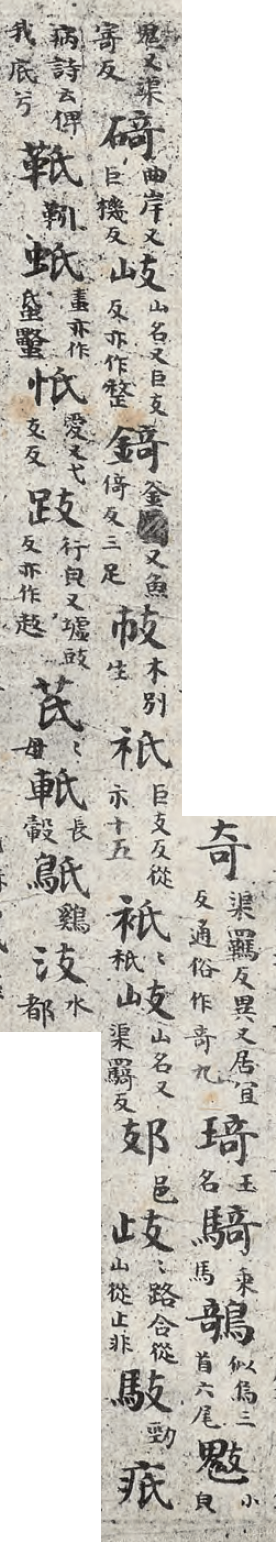
\includegraphics[height=1.46\textwidth]{Chapter5/gje.png}
    \caption{The homophone groups 奇 \textit{gje} and 祁 \textit{gjie} from the 刊謬補缺切韻 \textit{Kānmiù Bǔquē Qièyùn} of 706 CE.}
    \label{fig:Wang-gje-and-gjie}
\end{figure}

\begin{figure}[p]
\begin{adjustbox}{max width=1.3\textwidth,center}
    \centering
        \begin{tabular}{ll}
Transcription & Translation \\
\makecell[l]{{\large 奇}
渠羈反, \\ 異又居宜反,
通俗作奇九}
& \makecell[l]{1. {\large 奇 \textit{gje}} (渠 \textit{gjo} + 羈 \textit{kje} ), 異 also pronounced \textit{kje} (居 \textit{kjo} + 宜 \textit{ngje}), \\ 
 the vulgar writing is 竒. \\ A total of nine characters have the pronunciation gje.}
\\
{\large 琦}玉名
& 2. {\large 琦} name of a precious stone. \\
{\large 騎}乘馬
& 3. {\large 騎} ride a horse.  \\
{\large 鵸}似烏,三首六尾
& 4. {\large 鵸} like a crow, with three heads and six tails. \\
{\large 鬾}小兒鬼又渠寄反
& 5. {\large 鬾} ghost of a small child; also pronounced 渠 \textit{gjo} + 寄 \\
{\large 碕}曲岸又巨機反
& 6. {\large 碕} curved shore, also pronounced \textit{g{\sil{jɨj}}} (巨 \textit{gjoX} + 機 \textit{{\sil{kjɨj}}}). \\
{\large 岐}山名又巨支反亦作
& \makecell[l]{7. 岐 name of a mountain; also pronounced \textit{gje} (巨gjoX+支tsye); \\ also written .} \\
{\large 錡}釜屬又魚倚反三足 
& 8. {\large 錡} a type of cauldron; also pronounced ngjeX (魚 ngjo+倚 'jeX), with three legs.\\
{\large ��}木別生
& 9. {\large ��} [something] growing separately [from] a tree', [i.e. an arboreal parasite.] \\
& \\
{\large 祁}巨支反從示十五
& \makecell[l]{1. {\large 祁} \textit{gjie} (巨 \textit{gjoX} + 支 \textit{tsye}), from 示 'spirit'. \\ A total of fifteen characters have the pronunciation \textit{gjie}.} \\
{\large 衹}〻秖
& 2. {\large 衹} The first syllable of 衹秖 'monastic robes'. \\
{\large 岐}山名又渠羈反
& 3. {\large 岐} name of a mountain; also pronounced \textit{gje} (渠 \textit{gjo} + 羈 \textit{kje}). \\
{\large ��}邑
& 4. {\large ��} town (邑).\\
{\large 歧}〻路合從山從止非
& 5. {\large 歧} crossroad. From 山 not from 止. \\
{\large 馶}勁
& 6. {\large 馶} strong (勁). \\
{\large 疧}病《詩》云「俾我底兮」 
& 7. {\large 疧} sick; the Odes say 俾我底兮 'makes me sick!' \\
{\large ��}靷
& 8. {\large ��} leather belt that connects a horse with a cart (靷). \\
{\large 蚔}䖯亦作��
& 9. {\large 蚔} poisonous insect (䖯), also written �� and. \\
{\large 忯}愛又弋支反
& 10. 忯 love; also pronounced \textit{ye}  (弋 \textit{yik} + 支 \textit{tsye}) \\
{\large 跂}行兒又墟豉反亦作䞚
& \makecell[l]{11. 跂 walk like a child (i.e. crawl); also pronounced \textit{khje} (墟 \textit{khjo} +豉 \textit{dzye}), \\ also written 䞚.} \\
{\large 芪}〻母
& 12. {\large 芪} first syllable of 芪母, a kind of medicinal grass. \\
{\large 軝}長轂
& 13. {\large 軝} protruding part of a hub (長轂). \\
{\large 䲬}鷄
& 14. {\large 䲬} chicken (鷄). \\
{\large 汥}水都
& 15. {\large 汥} aggregation of water.
        \end{tabular}
\end{adjustbox}
\caption{The homophone groups 奇 \textit{gje} and 祁 \textit{gjie} from the 刊謬補缺切韻 \textit{Kānmiù Bǔquē Qièyùn} of 706 CE. (A transcription and translation of \ref{fig:Wang-gje-and-gjie})}
\end{figure}


\begin{description} \item
可 \emph{khaX} = 枯 \emph{kh}(\emph{u})+ 我 (\emph{ng})\emph{aX}
\item
枯  \emph{khu} = 苦  \emph{kh}(\emph{uX})+ 胡 (\emph{h})\emph{u}
\item
苦  \emph{khuX} = 康  \emph{kh}(\emph{ang}) + 杜 (\emph{d})\emph{uX}
\item
康 \emph{khang} = 苦  \emph{kh}(\emph{uX}) + 岡 (\emph{k})\emph{ang}
\item
空 \emph{khuwng} = 苦  \emph{kh}(\emph{uX}) + 紅 (\emph{h})\emph{uwng}
\item
楷  \emph{khojX} = 苦  \emph{kh}(\emph{uX}) + 駭 (\emph{h})\emph{ojX}
\item
口 \emph{kuwX} = 苦  \emph{kh}(\emph{uX}) + 後 (\emph{h})\emph{uwX}
\item
客 \emph{khæk} = 苦 \emph{kh}(\emph{uX}) + 格 (\emph{k})\emph{æk}
\end{description}


The result of applying this method to all  \emph{fǎnqiè} onset spellers
in the \emph{Qièyùn} is 51 chains of  \emph{fǎnqiè} onset spellers (聲類
 \emph{shēnglèi}). These onset classes are not phonemes, but merely
chains of onset \emph{fǎnqiè} spellers assembled philologically. The
 \emph{Qièyùn} is silent on the phonetic value of these 51 onset classes.
For their phonetic value we turn to the rime tables.

The  \emph{Yùnjìng} explicitly distinguishes initials into place and
manner of articulation with terms such as labial (唇 \emph{chún}),
dental (舌 \emph{shé}), voiceless (清 \emph{qīng}), voiceless aspirated
(次清 \emph{cìqīng}), etc. the \emph{Qīyīnlüè} distinguishes 36 initials
by giving an example of each.\footnote{The preface to the  \emph{Yùnjìng}
  contains a list of the same list of 36 initials, but the body of the
  text does not classify characters according to these initials.} Thus,
what the  \emph{Yùnjìng} describes as a `voiceless labial' the
 \emph{Qīyīnlüè} refers to acrophonically as the 幫 \emph{p}(\emph{ang})
initial. Whereas associating sounds with the 51 onsets of the
 \emph{Qièyùn} on the basis of internal evidence is not possible,
associating sounds with the 36 initials of the \emph{Qīyīnlüè} and the
articulatory categories of the \emph{Yùnjìng} is feasible. Hereafter I
refer to `the rime tables' when the distinction between the
 \emph{Yùnjìng} and the the \emph{Qīyīnlüè} is clear or unimportant.

Some effort must be taken to reconcile the 36 rime table initials of
relatively known phonetic interpretation with the  \emph{Qièyùn}'s 51
onsets of unknown phonetic value. There are cases where the rime tables
split cat­e­gories which can be linked in the  \emph{Qièyùn} and cases
where the rime tables conflate categories which cannot be linked in the
 \emph{Qièyùn} (\cite[45-61]{Baxter1992}, 
 \cite[14-16]{Baxter2014OldChinese}). The
splits reflect conditioned changes in the pronunciation of Chinese
during the centuries intervening the composition of the the works in
question and need concern us no further here.\footnote{The 9th century
  Buddhist monk 守溫 Shǒuwēn is traditionally credited with enumerating
  the 36 initials, but fragments from 敦煌 Dūnhuáng potentially
  creditable to him enumerate only 30 initials (\cite[206-207]{Pulleyblank1970LateMC}, 
  \cite{Coblin2006reflections}). The 30 initials omit some of the subsequent
  innovations. In particular, the the labiodental fricatives
  (\emph{qīngchún} 輕唇), viz. 非 f-, 敷 fh, 奉 v-, 微 ɱ- of the later
  36-initials \citep[41, 46-47]{Baxter1992}
  are not listed in the 30
  initials, although the fragment may show an awareness of their
  distinct pronunciation (\cite[210]{Pulleyblank1970LateMC}, 
  \cite[118]{Coblin2006reflections}). }
The latter cases, in which the rime tables collapse categories distinct
in the \emph{Qièyùn}, are of interest because the rime tables may
correctly subsume under one initial category  \emph{fǎnqiè} onset chains
that are in com­ple­men­tary distribution with respect to \emph{Qièyùn}
rime categories. Let us consider two examples \citep[112-114]{Tang2002}. 

In the first example the rime tables categorize some characters as
having the 照母 \emph{zhàomǔ} initial (here provisionally written
 \emph{č}-) which the \emph{Qièyùn} puts in the distinct \emph{fǎnqiè}
chains 側莊阻鄒簪仄爭 and 之職章諸旨止脂征正占支煮 (here provisionally
distinguished as \emph{č{\sil{₁}}- } and \emph{č{\sil{₂}}- } respectively); see . The
initials \emph{č{\sil{₁}}}- and \emph{č{\sil{₂}}}- must be considered distinct because
there are some rime categories com­patible with both, in particular
-\emph{ik} (\emph{zhí~}職 \emph{~tsyik}), -\emph{jang
}(\emph{yáng~}陽 \emph{~yang}), and -\emph{jo
}(\emph{yú~}魚 \emph{~ngjo}), i.e.  \emph{č{\sil{₁}}}- and \emph{č{\sil{₂}}}- are not in
com­ple­men­tary distribution with respect to the  \emph{Qièyùn} rime
categories. Thus, in his transcription system Baxter distinguishes
 \emph{tsr}- (pro­vi­sional \emph{č{\sil{₁}}}-) and \emph{tsy}- (provisional
 \emph{č{\sil{₂}}}-).


\begin{figure}[t]
\centering
\begin{minipage}[c]{\textwidth}
\centering
        \begin{tabular}{lllll}
\multicolumn{2}{l}{fǎnqiè onset speller (its rime)}
 &&
\multicolumn{2}{l}{fǎnqiè onset speller (its rime)} \\
側 \textit{č{\sil{₁}}ik} &
(\textit{zhí} 職 \textit{tsyik}) &&

之 \textit{č{\sil{₂}}i } &
(\textit{zhī} 之 \textit{tsyi}) \\
莊 \textit{č{\sil{₁}}jang} & 
(\textit{yáng} 陽 \textit{yang})\footnote{The reading of the character 莊 č{\sil{₁}}jang is described as an initial voiceless affricate (齒音 chǐyīn, 清 qīng) on chart 31 of the Yùnjìng and as initial č- (照 zhào) on chart 34 of the Qīyīnlüè. \\
}
&&

職 \textit{č{\sil{₂}}ik} &
(\textit{zhí} 職 \textit{tsyik}) \\
阻 \textit{č{\sil{₁}}joX} &
(\textit{yú} 魚 \textit{ngjo})&&

章 \textit{č{\sil{₂}}jang} &
(\textit{yáng} 陽 \textit{yang}) \\
鄒 \textit{č{\sil{₁}}juw} &
(\textit{yóu} 尤 \textit{hjuw}) &&

諸 \textit{č{\sil{₂}}jo} &
(\textit{yú} 魚 \textit{ngjo}) \\
簪 \textit{č{\sil{₁}}im} &
(\textit{qīn} 侵 \textit{tshim}) &&

旨 \textit{č{\sil{₂}}ijX} &
(\textit{zhī} 脂 \textit{tsyij}) \\
仄 č{\sil{₁}}ik  &
(\textit{zhí} 職 \textit{tsyik}) &&

止 \textit{č{\sil{₂}}iX} &
(\textit{zhī} 之 \textit{tsyi})\footnote{The reading of the character 止 č{\sil{₂}}iX is described as an initial voiceless affricate (齒音 shéchǐ, 清 qīngzhuó) on chart 8 of the Yùnjìng and as č- (照 zhào) on chart 8 of the Qīyīnlüè.}
\\
爭 \textit{č{\sil{₁}}eang}  &
(\textit{gēng} 耕 \textit{keang}) &&

脂 \textit{č{\sil{₂}}ij}  &
(\textit{zhī} 脂 \textit{tsyij}) \\

&&&

征 \textit{č{\sil{₂}}eng}  &
(\textit{qīng} 清 \textit{tshjeng}) \\

&&&

正 \textit{č{\sil{₂}}eng} &
 (\textit{qīng} 清 \textit{tshjeng}) \\

&&&

占 \textit{č{\sil{₂}}em}  &
(\textit{yán} 鹽 \textit{yem}) \\

&&&

支 \textit{č{\sil{₂}}e}  &
(\textit{zhī} 支 \textit{tsye}) \\

&&&

煮 \textit{č{\sil{₂}}joX}  &
(\textit{yú} 魚 \textit{ngjo})\\
\end{tabular}        \caption{The fǎnqiè onset speller chains  č{\sil{₁}}- and č{\sil{₂}}-, 
distinguishable in the \textit{Qièyùn} but not in the rime tables}
    \label{fig:fanqiec1c2}
\end{minipage}
\end{figure}

In the second example the rime tables categorize characters as having
the 來母 \emph{láimǔ} initial (here provisionally written \emph{l}-)
which the \emph{Qièyùn} puts in the distinct  \emph{fǎnqiè} chains
盧郎落魯來洛勒賴練 and 力良呂里林離連縷 (here provisionally
distinguished as \emph{l{\sil{₁}}- }and \emph{l{\sil{₂}}- }respectively); see . In this
case there are no rimes that occur in both  \emph{fǎnqiè} onset chains.
Thus, the rimes themselves sufficiently index the two types of
 \emph{l}-. The two are in complementary distribution and may be
re­gard­ed as allophones of the same phoneme (perhaps a `light l' and a
'dark l'). Because of their complementary distribution, Baxter's
transcription uses \emph{l}- for the Middle Chinese pro­nun­ci­a­tions
of characters written with both \emph{fǎnqiè} chains.\footnote{I have
  taken a methodologically unwarranted short cut. What I show here is
  that the rhymes of the initial \emph{fǎnqiè} spellers themselves are
  in complementary distribution, but better would be to show that all of
  the rimes in which words spelled with these spellers occur are in
  complementary distribution.}

By testing in this way all pairs of  \emph{fǎnqiè} onset chains in the
 \emph{Qièyùn} that are not assigned by the rime tables to distinct
initials, as to whether or not the two chains are in complementary
distribution relative to \emph{Qièyùn} rime categories, one reduces the
51 distinct  \emph{fǎnqiè} onset chains to 42 distinct  \emph{Qièyùn}
initials (聲母~ \emph{shēngmǔ}), as presented in .\footnote{The terms in
  are not necessarily those of any particular primary source, but
  instead are traditional in the teaching of Middle Chinese phonology.
  Although there is no traditional Chinese name for initial  \emph{zr}-,
  I herein refer to it as 俟  \emph{sì}
  \citep[15-46]{Baxter2014OldChinese}.}

The reader may protest that by observing the patterns of distribution
between the 51  \emph{fǎnqiè} onset chains in the  \emph{Qièyùn} and the
193 rime categories of the  \emph{Qièyùn}, one could establish without
reference to the rime tables that the  \emph{fǎnqiè} onset chain of which
盧 \emph{lú} is a member and that of which 力~ \emph{lì }is a member can
be united, whereas the chains of which 側 \emph{cè }and 之 \emph{zhī}
are respectively members cannot be. This al­ter­na­tive method, reducing
the 51  \emph{fǎnqiè} onset chains to a smaller number of distinct
initial cate­gories while ignoring the rime tables avoids the
anachronism of using a book from 1161 to analyze the categories of a
book from 601. Nonetheless, the alternative method has the practical
disadvantage of arriving at a number of initials lower than 42 which
the entire edifice of historical Chinese linguistics operates with.
Although conceptually this is an advantage, since it demonstrates that
the the rime tables distort one's perception of the  \emph{Qièyùn}, and
one may express the hope that in the future the 42 initials will be
abandoned as the dross of tradition, to propose an alternative analysis
here would take us well beyond the scope of this work's intended scope
and potentially confuse the student uniformly finds 42 initials
discussed in other works. To give an example, initials 泥 \emph{n}- and
娘 \emph{nr}-, although in com­ple­men­tary distribution, are usually
regarded as distinct Middle Chinese initials because they are
dis­tin­guished in the rime tables .\footnote{Note that 30
  initials of the Dūnhuáng fragments (see note ) omit initial 娘
  \emph{nr-}. Initials 匣 \emph{h-} and 雲 \emph{hj-} (the latter a
  subset of the 喻 yù initial category of the rime tables) are
  also in complementary distribution.}

The true drawback of ignoring the rime tables is that one then loses the
phonetic information that the two  \emph{fǎnqiè} onset chains which 盧
 \emph{lú} and 力 \emph{lì} respectively belong to are classed in the
rime tables as having an initial liquid resonant (舌齒 \emph{shéchǐ},
清濁 \emph{qīngzhuó}) or lateral (來目  \emph{láimù}) and that the two
chains which 側 \emph{cè} and 之 \emph{zhī} respectively belong to are
classed in the rime tables as having an initial voiceless affricate
(齒音 \emph{shéchǐ}, 清 \emph{qīngzhuó}) or 照母  \emph{zhàomǔ} initial.

\begin{figure}[t]
\centering
\begin{minipage}[c]{\textwidth}
\centering
        \begin{tabular}{lllll}
\multicolumn{2}{l}{fǎnqiè onset speller (its rime)}
 &&
\multicolumn{2}{l}{fǎnqiè onset speller (its rime)} \\
盧 \textit{l{\sil{₁}}u} & (\textit{mó} 模 \textit{mu}) &&
力 \textit{l{\sil{₂}}ik} & (\textit{zhí}  職 \textit{tsyik}) \\
郎 \textit{l{\sil{₁}}ang} &
(\textit{táng} 唐 \textit{dang}) && 
良 \textit{l{\sil{₂}}jang} &
(\textit{yáng} 陽 \textit{yang}) \\

落 \textit{l{\sil{₁}}ak} &
(\textit{duó} 鐸 \textit{dak}) &&

呂 \textit{l{\sil{₂}}joX} & 
(\textit{yú} 魚 \textit{ngjo}) \\

魯 \textit{l{\sil{₁}}uX}  &
(\textit{mó} 模 \textit{mu}) &&

里 \textit{l{\sil{₂}}iX} &
(\textit{zhī} 之 \textit{tsyi}) \\

來 \textit{l{\sil{₁}}oj} &
(\textit{hāi} 咍 \textit{xoj}) &&

林 \textit{l{\sil{₂}}im} &
(\textit{qīn} 侵 \textit{tshim}) \\

洛 \textit{l{\sil{₁}}ak} &
(\textit{duó} 鐸 \textit{dak}) &&

離 \textit{l{\sil{₂}}je} &
(\textit{qí} 齊 \textit{tsij}) \\


勒 \textit{l{\sil{₁}}ok}  &
(\textit{dé} 德 \textit{tok}) &&

連 \textit{l{\sil{₂}}jen} &
(\textit{xiān} 仙 \textit{sjen})\footnote{The reading of the character 連 \textit{l{\sil{₂}}jen} (\textit{xiān} 仙 \textit{sjen}) is described as a initial liquid resonant (舌齒 \textit{shéchǐ}, 清濁 \textit{qīngzhuó}) on chart 23 of the \textit{Yùnjìng} (Figure 17) and as l- (來 \textit{lái}) on chart 23 of the \textit{Qīyīnlüè} (Figure 18).} \\

賴 \textit{l{\sil{₁}}ajH} &
(\textit{tài} 泰 \textit{thajH}) &&

縷\textit{ l{\sil{₂}}juX} &
(\textit{yú} 虞 \textit{ngju}) \\

練 \textit{l{\sil{₁}}enH} &
(\textit{xiān} 先 \textit{sen})\footnote{The reading of the character 練 \textit{l{\sil{₁}}enH} is described as a initial liquid resonant (舌齒 \textit{shéchǐ}, 清濁 \textit{qīngzhuó}) on chart 23 of the \textit{Yùnjìng} (Figure 17) and as l- (來 \textit{lái}) on chart 23 of the \textit{Qīyīnlüè} (Figure 18).} &&& 

\end{tabular}        \caption{The fǎnqiè onset speller chains  \textit{l{\sil{₁}}}- and \textit{l{\sil{₂}}}-,  distinguishable in the Qièyùn but not in the rime tables}
    \label{fig:fanqiel1l2}
\end{minipage}
\end{figure}

\paragraph{The `ranks' of the rime tables and
`divisions' of the
 \emph{Qièyùn}.} Without explanation the rime tables
classify rimes among four 等~ \emph{děng} `ranks'. These `ranks' refer
fundamentally to the \emph{mise-en-page} of these two particular
documents, each rank corresponding to a row on a page. Although the
linguistic meaning of these `ranks' is obscure, they bear certain
relationships with dis­tri­bu­tional classes of co-occurrences between
initials and rimes in the \emph{Qièyùn} (\cite[7]{Schuessler2009minimal}, 
\cite[]{Shen2017}). In English it is useful to distinguish between `rank' as
the term for the four rows of the rime tables and `division' for the
analogous but distinct categories in the  \emph{Qièyùn}, even though the
Chinese term 等~ \emph{děng} is the same in both cases 
\citep[13]{Shen2017}. The paraphrase of `ranks' into `divisions' proceeds in two
steps. Jiāng Yǒng 江永 (1681-1762) took the first step in his 四聲切韻表
 \emph{Sìshēng Qièyùnbiǎo}; he looked up characters in each \emph{Qièyùn
}rime category to see which `rank' the rime tables place them in. Using
this procedure the rime categories of the  \emph{Qièyùn} divide into four
classes: (1) rimes that contain characters appearing in rank-i only, (2)
rimes that contain characters appearing in rank-ii only, (3) rimes that
contain mostly characters that appear in rank-iii, but containing some
characters appearing in rank-ii or rank-iv, (4) rimes that contain only
characters put into rank-iv (Shen Ruiqing 2017: 16). These classes of
rimes we may respectively dub `division-i rimes', `division-ii rimes',
'division-iii rimes', and `division-iv rimes'.\footnote{One explanation
  for the appearance of division-iii rimes in rank-ii is the sound
  change \emph{Tsrj}- \textgreater{} \emph{Tsr}- (cf. 
  \cite[267-269, 580-581]{Baxter1992}.} These `divisions' are hybrid beasts, with the rime
categories of the  \emph{Qièyùn} and the ranks of the rime tables as
their parents. In the second step, the realization that the divisions so
defined mostly coincide with dis­tri­bu­tional classes of  \emph{Qièyùn}
initials allows one to redefine the divisions using these co-occurence
patterns, and thereby avoid referring to rime table ranks. Rimes of all
four divisions occur with laryngeal (\emph{hóu} 喉 \emph{H}-), velar
(\emph{yá} 牙 \emph{K}-), and labial initials (\emph{chún }唇
 \emph{P}-). Retroflex stops (\emph{shéshǎng} 舌上 \emph{Tr}-) and
retroflex sibilants (\emph{zhuāngzǔ} 莊組  \emph{Tsr}-) initials occur
only with division-ii rimes; initial 來 \emph{l}- does not occur with
division-ii rimes. Palatal initials (\emph{zhāngzǔ} 章組 \emph{Tsy}-)
occur only with division-iii rimes.\footnote{If these co-occurrence
  patterns were articulated in terms of distinct  \emph{fǎnqiè} onset
  chains (聲類 \emph{shēnglèi}) instead of with initials
  (聲母~ \emph{shēngmǔ}), one could further observe that \emph{l{\sil{₂}}}- only
  occurs with division-iii rimes.} Dental initials (\emph{shétóu} 舌頭
 \emph{T}-) occur only with division-i and division-iv rimes. In fact,
rimes of division-i and division-iv pattern identically with regard to
their co-occurence with initials.\footnote{Most Chinese dialects show a
  prevocalic glide in division-iv words, e.g. 牽 Mandarin \emph{qiān}
  \textless{} MChi. \emph{khen. }The presence of this medial is
  presumably the reason the rime tables place these words in division-iv
  rather than division-i. Baxter argues that this medial arose due to a
  sound change affecting inherited front vowels between the composition
  of the  \emph{Qièyùn} and the composition of the rime tables 
  \citeyearpar[241-243]{Baxter1992}.} Thus, from the perspective of the  \emph{Qièyùn} it is
impossible to distinguish between division-i and division-iv; they can
be treated as a single division-i/iv (see ).

These statements of attested co-occurrence between a class of rimes and
a class of initials may be understood as the defining criteria of the
three divisions (viz. i/iv, ii, and iii) based on the internal evidence
of the \emph{Qièyùn.} In other words, the unsatisfactory
characterization of the ranks as an idiosyncrasy of the page formatting
of the rime tables is thus paraphrasable as linguistically meaningful
dis­tri­bu­tional classes in the  \emph{Qièyùn}.

\begin{figure}
    \centering
\begin{tabular}{|lr|l|l|l|l|l|l|l|}
\hline
唇音 & P- &  
幫 \textit{p-} &
滂 \textit{ph-} &
並 \textit{b-} &
明 \textit{m-} &&&
\\ \hline
舌頭音 & T- &
端 \textit{t-} &
透 \textit{th-} &
定 \textit{d-} &
泥 \textit{n-} &&&
\\ \hline
舌上音 & Tr- &
知 \textit{tr-} &
徹 \textit{trh-} &
澄 \textit{dr-} &
娘 \textit{nr-} &&&
\\ \hline
齒頭音 & Ts- &
精 \textit{ts-} &
清 \textit{tsh-} &
從 \textit{dz-} &
&
心 \textit{s-} &
邪 \textit{z-} &
\\ \hline
莊組 & Tsr- &
莊 \textit{tsr-} &
初 \textit{tsrh-} &
崇 \textit{dzr-} &
&
生 \textit{sr-} &
俟 \textit{zr-} &
\\ \hline
章組 & Tsy- &
章 \textit{tsy-} &
昌 \textit{tsyh-} &
禪 \textit{dzy-} &
日 \textit{ny-} &
書 \textit{sy-} &
船 \textit{zy-} &
以 \textit{y-} \\ \hline
牙音 & K- &
見 \textit{k-} &
溪 \textit{kh-} &
群 \textit{g-} &
疑 \textit{ng-} &
&& \\ \hline


喉音 &&
影 \textit{'-} &
曉 \textit{x-} &
匣 \textit{h-} &
&&&
云 \textit{hj-}
\\ \hline
半舌音 &&
來 \textit{l-} &&&&&& \\
\hline
\end{tabular}
    \caption{The 42 initials of the Qièyùn 
    \citep[15]{Baxter2014OldChinese}}
    \label{fig:34-initials}
\end{figure}

\begin{figure}
    \centering
    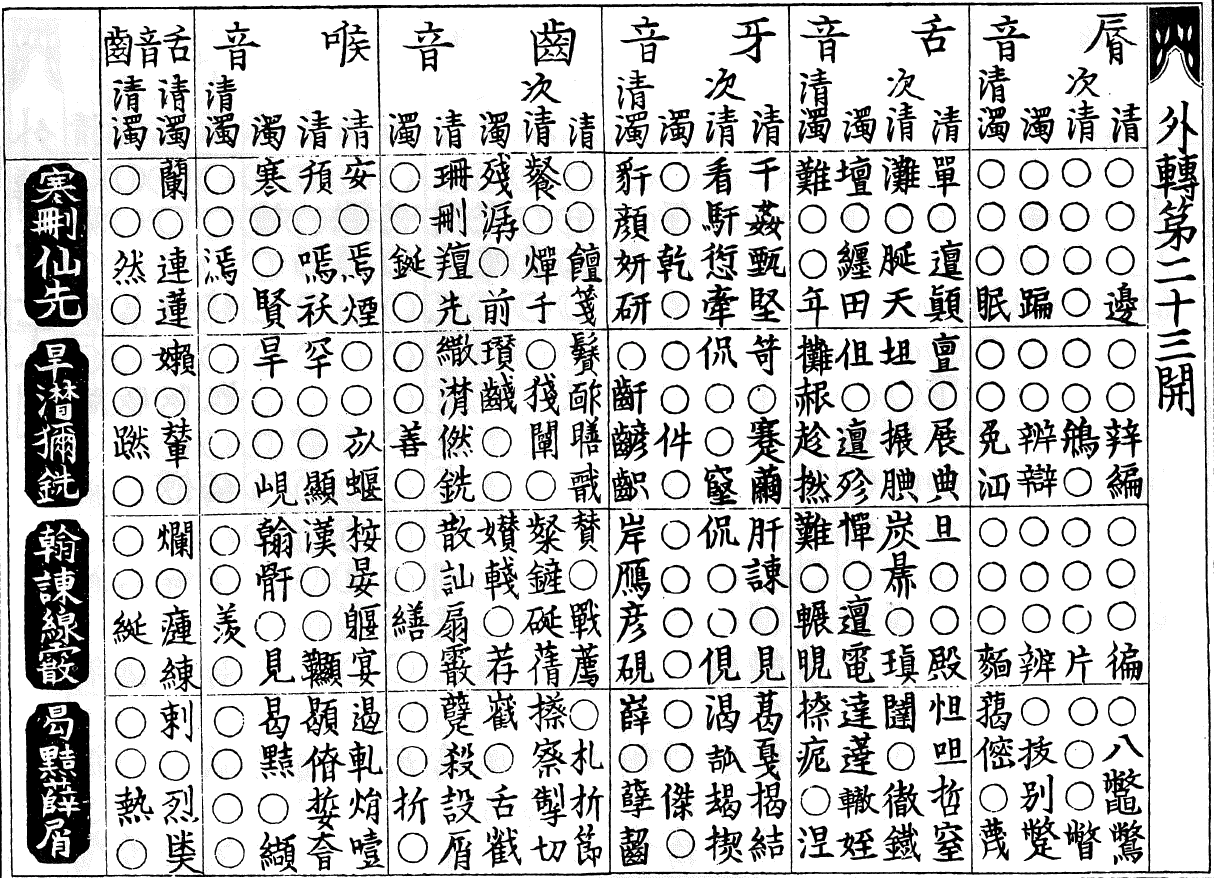
\includegraphics[width=1\textwidth]{Chapter5/fig17 Yunjing 23 version 1.png}
    \caption{Chart 23 from the \textit{Yùnjìng}}
    \label{fig:Yunjing23}
\end{figure}

A more thoroughgoing presentation of the co-occurrence restrictions of
the initial classes with rimes further permits division-i/iv and
division-ii to be collapsed. Division-i/iv rimes occur with dental
(\emph{shétóu} 舌頭 \emph{T}-) and affricate initials (\emph{chǐtóu}
齒頭 \emph{Ts}-) but not with retroflex (\emph{shéshǎng} 舌上
 \emph{Tr}-) or retroflex affricate (\emph{zhuāngzǔ} 莊組 \emph{Tsr}-)
initials. Division-ii occurs with retroflex (\emph{shéshǎng} 舌上
 \emph{Tr}-) and retroflex affricates (\emph{zhuāngzǔ}~莊組 \emph{Tsr}-)
but not with dental (\emph{shétóu} 舌頭  \emph{T}-) or affricate
(\emph{chǐtóu} 齒頭~ \emph{Ts}-) initials. Thus, division-i/iv is in
com­ple­men­tary distribution with division-ii; those places where the
one is allowed the other is forbidden, although both are forbidden from
the palatals (\emph{zhāngzǔ} 章組  \emph{Tsy}-). This com­ple­men­tary
distribution permits division-i/iv and division-ii to be united. From
this new perspective division-i/iv/ii bears the name `type A' and
division-iii bears the name `type B' (see ). The dis­tri­bu­tional
categories of the  \emph{Qièyùn} itself permit analysis either in terms
of the three division-i/iv, division-ii, and division-iii or of the two
types A and B. Whether one speaks of divisions or types is simply a
question of which dis­tri­bu­tional facts are in focus. Both ways of
looking at the co-occurence of initial categories with rime categories
are syn­chron­i­cally true of Middle Chinese as reflected in the
 \emph{Qièyùn}. Nonetheless, in practice the terminology of `divisions'
in used with reference to Middle Chinese and the terminology of `types'
is used with reference to Old Chinese.

\begin{figure}
    \centering
    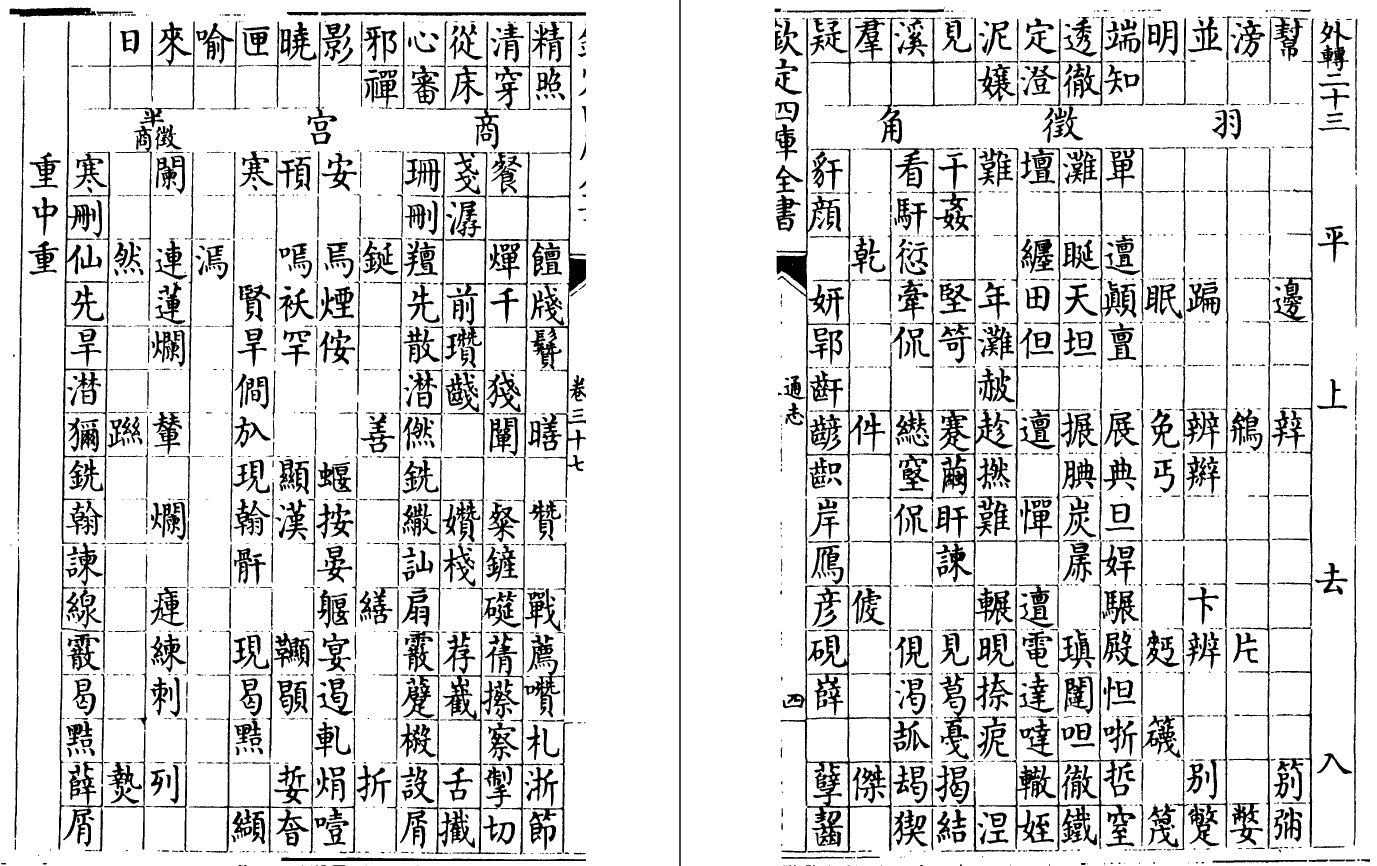
\includegraphics[width=1\textwidth]{Chapter5/fig18 Qiyinlue 23 version 1.png}
    \caption{Chart 23 from the \textit{Qīyīnlüè}}
    \label{fig:Qinyinlue23}
\end{figure}


In Baxter's Middle Chinese notation division-ii rimes are marked with
the vowels -\emph{ea}- and -\emph{ae}- and division-iii rimes are marked
with a main vowel -i- or pre-vocalic -j- (orthographically omitted after
initial palatals, i.e.  \emph{zhāngzǔ} 章組  \emph{Tsy}-) 
\citep[67-75]{Baxter1992}.\footnote{Note that in Baxter's system -\emph{ea}- occurs only in
  division-ii whereas -\emph{ae}- occurs in both division-ii and
  division-iii, so it is only in the absence of -\emph{j}- or -\emph{y}-
  in the onset that -\emph{ae}- by itself indexes division-ii.} The lack
of an indication of division-ii or division-iii using these conventions
itself indexes syllables of division-i/iv in Baxter's system; among
these syllables division-iv are indicated with the nuclear vowel
-\emph{e}-, whereas division-i syllables occur with -\emph{a}-,
-\emph{u}-, or -\emph{o}-. Following a suggestion of
\citet[]{Norman1994},
Baxter \& Sagart posit pharyn­geal­iza­tion in Old Chinese as the origin
of type A syllables and non-pharyngealization as the origin of type B
syllables 
\citeyearpar[68-76]{Baxter2014OldChinese}. For the present purposes this hypothesis can be
viewed as a mechanical rewriting of Middle Chinese syllables without -j-
as Old Chinese syllables with -{\sil{ˤ}}- (not applied to syllables with the
main vowel -i-) and the concomitant omission of -j- in the Old Chinese
ancestors of Middle Chinese words that contain -j-.\footnote{To the
  extent that one relies on late sources such as the  \emph{Guǎngyùn},
  the post-\emph{Qièyùn} sound change *TSrj \textgreater{} TSr-
  complicates this otherwise mechanical rewriting
  \citep[53-54]{Baxter1992}.}

\begin{figure}
    \centering
\begin{tabular}{|l|l|l|l|l|l|l|}
\hline
     &  l- & T- & Tr- & Ts- & Tsy- & Tsr- \\
\hline
Division-i & {\sil{✓}} & {\sil{✓}} && {\sil{✓}} && \\
\hline
Division-ii & & & {\sil{✓}} & & & {\sil{✓}} \\
\hline
Division-iii & {\sil{✓}} && {\sil{✓}} && {\sil{✓}} & {\sil{✓}} \\
\hline
Division-iv & {\sil{✓}} & {\sil{✓}} && {\sil{✓}} && \\
\hline
\end{tabular}
    \caption{Co-occurrence of rimes of the four divisions with various types of Middle Chinese initials}
    \label{fig:co-occurence-of-divisions}
\end{figure}

\begin{figure}
    \centering
\begin{tabular}{|l|l|l|l|l|l|l|}
\hline
     &  l- & T- & Tr- & Ts- & Tsy- & Tsr- \\
\hline
Type-A & {\sil{✓}} & {\sil{✓}} & {\sil{✓}} & {\sil{✓}} && {\sil{✓}} \\
\hline
Type-B & {\sil{✓}} & & {\sil{✓}} & & {\sil{✓}} &  {\sil{✓}} \\
\hline
\end{tabular}
    \caption{Co-occurrence of the rimes of type A and B with various types of Middle Chinese initials}
    \label{fig:co-occurence-of-A-and-B}
\end{figure}


\paragraph{Medial -\emph{w}- (合口
 \emph{hékŏu}) according to the rime tables.}
The presence or absence of a medial -\emph{w}- in Middle Chinese is of
significance for the reconstruction of Old Chinese. Reference to the
 \emph{Qièyùn} alone does not allow for the identification of this
distinction. The rime tables make the distinction explicit. A given
table of the  \emph{Yùnjìng} (but not of the  \emph{Qīyīnlüè}) is labelled
on its far right as either entirely 合口  \emph{hékŏu} `closed mouth' or
開口 \emph{kāikŏu} `open mouth'.\footnote{In fact, the situation is more
  complex. First, some tables are labeled 開合  \emph{kāihé}. Second,
  modern textbooks more or less tacitly `correct' the primary sources.
  For example, 中 is treated as 合口  \emph{hékǒu} in textbooks, although
  it appears on chart 1 of  \emph{Yùnjìng}, which is labeled 開
   \emph{kāi}. Such discrepancies, seldom discussed explicitly, are in
  need of systematic and methodologically informed study. I thank Zev
  Handel for his help with this note and this entire chapter.} As these
terms themselves suggest, all re­searchers analyze the syllables
categorized under these rubrics as respectively with -\emph{w}- and
without -\emph{w}- (e.g, 
\cite[62]{Baxter1992},
\cite[9]{Schuessler2009minimal},
\cite[2013-204]{Baxter2014OldChinese}).

The \emph{hékŏu }versus \emph{kāikŏu} distinction is not contrastive
after labial initials, as revealed by the inconsistent placement of
labial initial words in the rime tables and inconsistent use of
 \emph{fǎnqiè} rime spellers (反切下字  \emph{fǎnqiè xiàzì}) with these
words in the \emph{Qièyùn}
\citep[62-63]{Baxter1992}.

\paragraph{The 重紐 \emph{chóngniǔ} problem.} Historical Chinese phonologists in the tradition of Karlgren
(1964{[}1957]) fill out the categories of the  \emph{Qièyùn} and rime
tables with phonetically meaningful alphabetic representations. In most
cases---rimes, initials,  \emph{hékŏu}/ \emph{kāikŏu}---the phonetic
terminology of the rime tables or a look at Chinese dialects immediately
suggests a phonetic interpretation of the philological category in
question. However, in one case, the so-called 重紐 `\emph{chóngniǔ}
problem', a distinction present in the  \emph{Qièyùn} resisted
confirmation and analysis for a long time.

As with other niceties of Middle Chinese phonology, the  \emph{chóngniǔ}
problem boils down to an observation about the  \emph{mise-en-page} of
the  \emph{Qièyùn} and the rime tables. The term `\emph{chóngniǔ'} means
'repeated button', where `button' refers to the dot that separates
homophone groups within the same rime category in the presentation of
rime books deriving from the  \emph{Qièyùn}. The extant fragments
indicate that the original edition of the  \emph{Qièyùn} did not use this
device 
\citep[36]{Bottero2013}. In the preface to the earliest complete
version, namely 王仁昫 Wáng Rénxù's 刊謬補缺切韻 \emph{Kānmiù Bǔquē
Qièyùn} of 706 CE, the author says that he will separate homophone
groups with red dots 
\citep[41]{Bottero2013}, but such dots are not visible
on the published facsimile 
\citep[434-527]{Zhou1983}. Nonetheless, even when
such dots are missing, one can notice a new homophone group where the
text gives a new  \emph{fǎnqiè} spelling followed by an explicit numeric
indication of the number of characters that fall into that particular
homo­phone group (see *****Figure 3.2 above).

Eight rimes of the \emph{Qièyùn} (viz. \emph{zhī} 支~-\emph{je},
 \emph{zhī} 脂~-\emph{ij},  \emph{zhài~}祭~-\emph{jejH},  \emph{xiāo}
宵~-\emph{jew},  \emph{qīn} 侵~-\emph{im},  \emph{yán} 鹽~-\emph{jem},
 \emph{zhēn} 真~-\emph{in}, and \emph{xiān} 仙~-\emph{jen}) contain a
pair of homo­phone groups that have in­com­men­surate chains of
 \emph{fǎnqiè} rime spellers and cannot be distinguished on the basis of
 \emph{hékŏu }versus \emph{kāikŏu} (Baxter 1977: 56, 60-64).

In general each homophone group of the  \emph{Qièyùn} corresponds to one
non-empty grid point in the rime tables. One may thus understand the
placement of a character in the tables as an acrophonic representation
of the table's treatment of all characters in the corresponding
 \emph{Qièyùn} homophone group. Looking at the treatment of pairs of
 \emph{chóngniǔ} homophone groups in the rime tables, the one homophone
group is put into rank-iii and the other group in rank-iv. As a matter
of terminology characters of a relevant  \emph{Qièyùn} homophone group
that is put in rank-iii are called `\emph{chóngniǔ} rank-iii' characters
(重紐三等  \emph{chóngniǔ sānděng}) and characters of the other
 \emph{Qièyùn} homophone group, the one put in rank-iv, are called
' \emph{chóngniǔ} rank-iv' characters (重紐四等  \emph{chóngniǔ sìděng}).
The pronunications of both types belong to division-iii (or equivalently
type B) in the sense that their lower  \emph{fánqiè} spellers are
division-iii.\footnote{More concretely, there is an overall tendency for
   \emph{chóngniǔ} rank-iii characters to have lower  \emph{fánqiè}
  spellers of rank-iii and for \emph{chóngniǔ} rank-iv characters to
  either have \emph{chóngniǔ} rank-iv lower  \emph{fánqiè} spellers or to
  have lower \emph{fánqiè} spellers of rank-iii with initials for which
  there are no \emph{chóngniǔ} distinctions.} In Baxter's transcription,
 \emph{chóngniǔ} rank-iv are marked with an additional i or j. For
instance, the \emph{chóngniǔ} rank-iii word 碑 he transcribes as
 \emph{pje }while the \emph{chóngniǔ} rank-iv word 卑 he transcribes as
 \emph{pjie}. It turns out that the \emph{chóngniǔ} problem only affects
characters of these eight rimes with labial (唇  \emph{chún}) or velar
(牙  \emph{yá}) initials.

Nothing in the \emph{Qièyùn} or rime tables draws attention to these
 \emph{chóngniǔ }homophone groups as special or worthy of comment. The
grounds for putting these characters in two different homo­phone groups
of the  \emph{Qièyùn} were obvious to the authors of that work and the
grounds for putting some characters of the one homophone group in
rank-iii and some characters of the other in rank‑iv were obvious to the
authors of the rime tables. However, because  \emph{chóngniǔ} doublet
homophone groups are in the same  \emph{Qièyùn} rime, the same rime table
column (i.e. have the same initial), because they match in being both
 \emph{kāikŏu} or both \emph{hékŏu}, because both have division-iii lower
 \emph{fánqiè} spellers, and because the readings of characters in both
groups are homo­phonous in all of the better known Chinese dialects, it
is difficult to see what part of the syllable is obviously
reconstructible as distinct for the two members of a pair. Thus, the
interpretation of these homophone groups is confounding and requires a
label to facilitate discussion.

Although the modern Chinese dialects do not generally allow a
distinction to be drawn between  \emph{chóngniǔ} rank-iii readings and
 \emph{chóngniǔ} rank-iv readings, plenty of evidence con­firms that the
phonetic distinction recorded in this distinction was real. For example,
in many cases the Ḥphags-pa script transcriptions of these characters in
the 14th century 蒙古字韻  \emph{Měnggǔ zìyùn} distinguishes
 \emph{chóngniǔ} rank-iii and \emph{chóngniǔ} rank-iv (\cite[]{Shen2005chongniu}); in this source 碑  \emph{pje} is transcribed
 
\includegraphics[width=0.25cm]{Chapter5/Phagspabue.png}
\textless{}bue\textgreater{} and 卑 \emph{pjie} is transcribed as
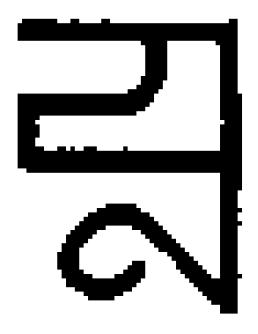
\includegraphics[width=0.25cm]{Chapter5/PhagspaBi.png}
\textless{}bi\textgreater{} (\cite[167]{Shen2005chongniu},
\cite[122 and 126]{Coblin2007}). Sino-Vietnamese character readings also provide evidence for
this distinction; 碑  \emph{pje} has the Sino-Vietnamese reading
 \emph{bi} whereas 卑 \emph{pjie} has the Sino-Vietnamese reading
 \emph{ti} 
 \citep[86]{Baxter1977}.
